%-------------------------------------------------------------------------------
% LATEX TEMPLATE ARTIKEL
%-------------------------------------------------------------------------------
% Dit template is voor gebruik door studenten van de de bacheloropleiding 
% Informatica van de Universiteit van Amsterdam.
% Voor informatie over schrijfvaardigheden, zie 
%                               https://practicumav.nl/schrijven/index.html
%
%-------------------------------------------------------------------------------
%	PACKAGES EN DOCUMENT CONFIGURATIE
%-------------------------------------------------------------------------------

\documentclass{uva-inf-article}
\usepackage[dutch]{babel}

\usepackage[style=authoryear-comp]{biblatex}
\addbibresource{references.bib}

\usepackage{soul}
\usepackage{xcolor}
\sethlcolor{yellow}

\usepackage{tikz}
\usetikzlibrary{arrows.meta, positioning}
\usepackage{float}
\usepackage{amsmath} 



%-------------------------------------------------------------------------------
%	GEGEVENS VOOR IN DE TITEL, HEADER EN FOOTER
%-------------------------------------------------------------------------------

% Geef je artikel een logische titel die de inhoud dekt.
\title{Governor Report}

% Vul de naam van de opdracht in zoals gegeven door de docent en het type 
% opdracht, bijvoorbeeld 'technisch rapport' of 'essay'.
\assignment{Assignment 3}
\assignmenttype{Report}

% Vul de volledige namen van alle auteurs in en de corresponderende UvAnetID's.
\authors{Matteo D'Urso; Adam Rakun;}
\uvanetids{16349210; 16339908;}

% Vul de naam van je tutor, begeleider (mentor), of docent / vakcoördinator in.
% Vermeld in ieder geval de naam van diegene die het artikel nakijkt!
\tutor{Hang Xu}
\mentor{}
\docent{Anuj Pathania}

% Vul hier de naam van je tutorgroep, werkgroep, of practicumgroep in.
\group{Group 11}

% Vul de naam van de cursus in en de cursuscode, te vinden op o.a. DataNose.
\course{Embedded Systems}
\courseid{5063EMSY6Y}

% Dit is de datum die op het document komt te staan. Standaard is dat vandaag.
\date{\today}

%-------------------------------------------------------------------------------
%	VOORPAGINA 
%-------------------------------------------------------------------------------

\begin{document}
\maketitle

%-------------------------------------------------------------------------------
%	INHOUDSOPGAVE EN ABSTRACT
%-------------------------------------------------------------------------------
% Niet toevoegen bij een kort artikel, zeg minder dan 10 pagina's!

%TC:ignore
%\tableofcontents
%\begin{abstract}
%\end{abstract}
%TC:endignore

%-------------------------------------------------------------------------------
%	INHOUD
%-------------------------------------------------------------------------------
% Hanteer bij benadering IMRAD: Introduction, Method, Results, Discussion.


\section{Introduction [0.5 Points]} 

% In the first assignment, you learned to set up the environment. In the second assignment, you developed a better understanding of your research problem by characterizing your
% hardware and software interactions. In the third and final assignment you will bring your project to a conclusion.
% You must now source your experience from previous assignments to create a power management solution for your design that is potentially better than the state-of-the-art. In this introduction section, explain your plan of action. It is important to link in the introduction to the
% observations in a second assignment that guide your design. It should be clear from
% the introduction as to why you gain improvements over the baseline (Example Governor). In other words, ex-
% plain what sub-optimalities you avoid present in the Example Governor and the additional optimizations you performed, which explains your results.
% \par\vspace{\baselineskip} 

This report describes the design and early results of an application-specific power governor for AlexNet inference on the Khadas VIM3 using the Pipe-All framework. The governor aims to minimize power consumption while satisfying user-specified throughput (FPS) and latency constraints, as required by the course specification.

In Assignment 2 we performed a power-performance characterisation of the platform and identified several trends that directly guided this governor design:
\begin{itemize}
  \item DVFS on both CPU clusters provides strong leverage over throughput/latency, but exhibits diminishing performance returns at the highest frequencies; mid-range DVFS points often provide better efficiency.
  \item Pipeline order and partition points can dominate behaviour: orders that place the Little CPU early tend to perform poorly for AlexNet, while GPU--Big--Little (G-B-L) is typically an efficient ordering.
  \item Very small pipeline stages can be counterproductive due to pipeline overhead (synchronization, buffering, and orchestration), sometimes reducing performance despite “using more components”. Because of that, we directly avoid having a single stage on one processing unit.
  \item Even for GPU-heavy execution, CPU frequencies impact system power due to CPU-side overhead (kernel launches, memory management, and synchronization).
\end{itemize}

\textbf{Plan of action:} \\
We use a hybrid approach that combines: \\
(1) a design-time initialization step that selects a promising starting configuration near the target (so we do not waste iterations exploring obviously suboptimal regions), and \\
(2) a run-time feedback PID controller that incrementally adjusts DVFS and partition points based on measured FPS/latency and on a lightweight power estimation model.

Compared to the Example Governor described in the course guide, our design avoids two major non-optimalities:
\begin{itemize}
  \item expensive brute-force exploration with full inference runs at every design point, and
  \item a purely monotonic heuristic that cannot trade off DVFS and partitioning in a coordinated way.
\end{itemize}

Instead, we: \\
(i) start from an empirically good “root” pipeline (G-B-L with partition points close to the efficient region seen in Assignment 2), \\
(ii) use a measurement-driven lookup approximation to seed the initial DVFS point, and \\
(iii) apply a multi-input multi-output (MIMO) control policy (implemented as two coupled PID loops) to approach feasibility quickly and then reduce power while preserving constraints.
 

\section{Design [0.75 Points]} 

%In this section, explain the design of your power management solution. It is highly recommended that you explain your design with as much visualization as possible. There are no constraints on the design but do provide the critical reasoning why you choose to do this particular design.

This section follows the same high-level structure as our presentation: Design-Time Lookup Initialization, Run-Time MIMO PID Control, PID Decisions, and Power Estimation Model.

\subsection{System architecture and control loop}

\begin{figure}[H]
\centering
\hspace*{-2cm}%
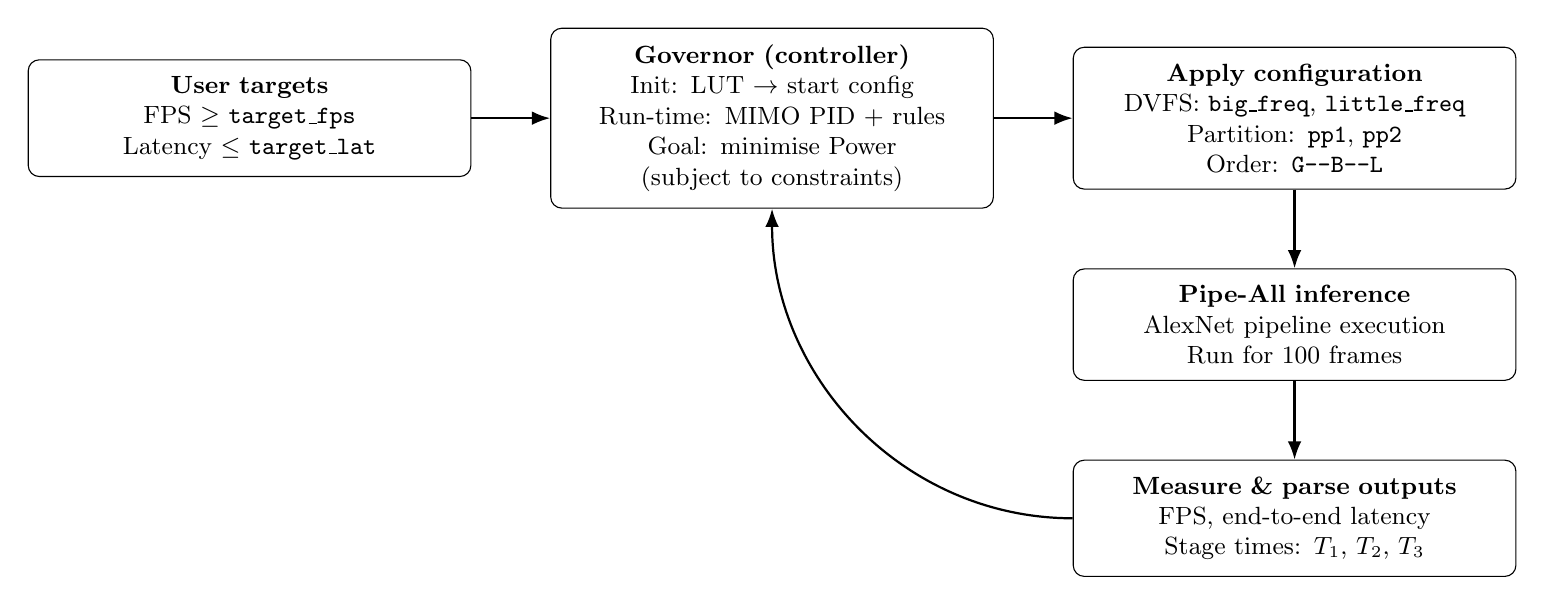
\begin{tikzpicture}[
    font=\small,
    box/.style={
      draw, rounded corners,
      align=center,
      text width=5.2cm,
      inner sep=6pt
    },
    arrow/.style={-Latex, thick},
    every node/.style={execute at begin node=\setlength{\hyphenpenalty}{10000}\setlength{\exhyphenpenalty}{10000}}
]

% --- Top row ---
\node[box] (targets) {\textbf{User targets}\\
FPS $\ge$ \texttt{target\_fps}\\
Latency $\le$ \texttt{target\_lat}};

\node[box, right=1.0cm of targets] (gov) {\textbf{Governor (controller)}\\
Init: LUT $\rightarrow$ start config\\
Run-time: MIMO PID + rules\\
Goal: minimise Power (subject to constraints)};

\node[box, right=1.0cm of gov] (apply) {\textbf{Apply configuration}\\
DVFS: \texttt{big\_freq}, \texttt{little\_freq}\\
Partition: \texttt{pp1}, \texttt{pp2}\\
Order: \texttt{G--B--L}};

% --- Bottom row ---
\node[box, below=1.0cm of apply] (system) {\textbf{Pipe-All inference}\\
AlexNet pipeline execution\\
Run for $100$ frames};

\node[box, below=1.0cm of system] (measure) {\textbf{Measure \& parse outputs}\\
FPS, end-to-end latency\\
Stage times: $T_1$, $T_2$, $T_3$};

% --- Arrows ---
\draw[arrow] (targets) -- (gov);
\draw[arrow] (gov) -- (apply);
\draw[arrow] (apply) -- (system);
\draw[arrow] (system) -- (measure);
\draw[arrow] (measure.west) to[out=180,in=-90] (gov.south);

\end{tikzpicture}

\end{figure}


The governor runs as a user-space C program that repeatedly:
\begin{enumerate}
  \item applies a candidate configuration (CPU frequencies + Pipe-All partition points + order),
  \item runs Pipe-All inference for a fixed number of frames,
  \item parses the output to extract measured FPS, latency, and per-stage inference times, and
  \item computes the next configuration using the controller.
\end{enumerate}

\par\vspace{\baselineskip}

\textbf{Key implementation components:}
\begin{itemize}
  \item \textit{Frequency control:} \texttt{set\_freq.sh} writes to \texttt{cpufreq} policy0 (Little) and policy2 (Big).
  \item \textit{Fan control:} \texttt{set\_fan.sh} sets a fixed fan mode to reduce power measurement variance.
  \item \textit{Inference execution:} \texttt{run\_inference.sh} runs the selected Pipe-All graph with $n$ frames and the chosen partition points and order.
  \item \textit{Parsing:} \texttt{parse\_results()} extracts FPS, latency, and stage inference times from the last run output.
\end{itemize}

\subsection{Design-Time: Lookup-based initialization}

Starting from a poor initial configuration increases convergence time, and can trigger unstable controller behaviour (large partition moves, frequent saturation at max frequencies). We therefore seed the initial DVFS point using a small pre-measured grid.
\par\vspace{\baselineskip}

\textbf{Implementation.} We load a CSV measurement grid produced during design-time frequency sweeps (fixed order and partition points). The function \texttt{approximate\_target\_space()} selects the $(f_\text{big}, f_\text{little})$ pair with minimal normalized constraint violation relative to the target, i.e. it tries to avoid underperforming configurations while keeping the initial point close to feasible.

\textbf{Assumption.} Because Assignment 2 showed that G-B-L order with mid-range partitioning tends to be efficient, we keep the order fixed to G-B-L and seed DVFS around an empirically strong partitioning (root configuration uses $pp1=4$, $pp2=6$). The controller then adjusts DVFS and partition points at run-time if the target requires it.

\subsection{Run-Time: MIMO PID controller (two coupled loops)}

We model the governor as a constrained optimization problem:

\begin{quote}
minimize $Power$\\
subject to $\ \hspace{1cm} \text{FPS} \ge \text{target\_fps}$\\
\hspace*{2.55cm} $\ \text{Latency} \le \text{target\_latency}$
\end{quote}

At run-time, we do not have direct measured power feedback (USB meter is external), so we minimize an estimated power model $P$ while using measured FPS/latency for feasibility.
\par\vspace{\baselineskip}

\textbf{Controller structure.} We implement two PID controllers:
\begin{itemize}
  \item \textbf{FPS PID:} acts when measured FPS is below target; primarily increases performance through DVFS and, if needed, partition adjustments.
  \item \textbf{Latency PID:} acts when measured latency exceeds target; primarily decreases end-to-end latency using DVFS and partition adjustments.
\end{itemize}

This is “MIMO” (multiple input - multiple output) in practice because both DVFS and partition points affect both FPS and latency; the controller therefore includes rule-based coupling logic that decides which knob to apply depending on which constraint is violated and which pipeline stage is the bottleneck.

Furthermore, we chose $K_p$, $K_i$, and $K_d$ to be slightly different values for the FPS PID and Latency PID Controller. Those values were found through trial and error. The results that we found, i.e. that $K_i$ is a little less agressive for Latency aligns with the findings from our previous research, as Latency responds stronger to change than FPS does and therefore has to be handled more gracefully. $K_p$ is the same for both controllers. $K_d$ was set to $0$ as the derivative term really can't handle noise well and the data that is provided by the inference run has a lot of noise. This renders our PID controller effectively a PI Controller but we continued to use the term PID Controller throughout code and report.

\begin{figure}[H]
\centering
\hspace*{-0.6cm}% move left (adjust to -0.4cm / -0.8cm if needed)
\resizebox{1.03\linewidth}{!}{% slight scale so spacing stays nice
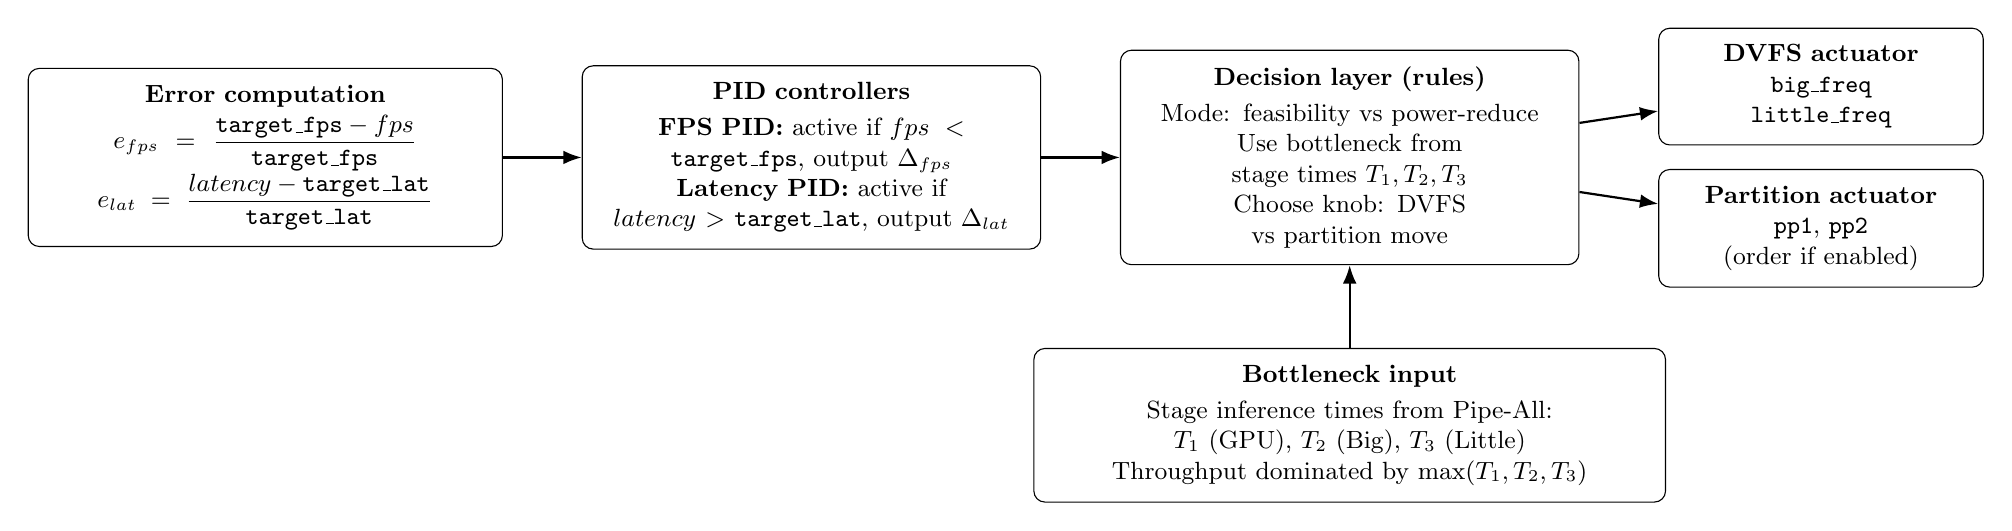
\begin{tikzpicture}[
    font=\small,
    box/.style={draw, rounded corners, align=center, inner sep=6pt},
    arrow/.style={-Latex, thick},
    every node/.style={execute at begin node=\setlength{\hyphenpenalty}{10000}\setlength{\exhyphenpenalty}{10000}}
]

% --- Blocks ---
\node[box, text width=5.6cm] (err) {\textbf{Error computation}\\[2pt]
$e_{fps}=\dfrac{\texttt{target\_fps}-fps}{\texttt{target\_fps}}$\\
$e_{lat}=\dfrac{latency-\texttt{target\_lat}}{\texttt{target\_lat}}$};

\node[box, text width=5.4cm, right=1.0cm of err] (pids) {\textbf{PID controllers}\\[2pt]
\textbf{FPS PID:} active if $fps < \texttt{target\_fps}$, output $\Delta_{fps}$\\
\textbf{Latency PID:} active if $latency > \texttt{target\_lat}$, output $\Delta_{lat}$};

\node[box, text width=5.4cm, right=1.0cm of pids] (dec) {\textbf{Decision layer (rules)}\\[2pt]
Mode: feasibility vs power-reduce\\
Use bottleneck from stage times $T_1,T_2,T_3$\\
Choose knob: DVFS vs partition move};

\node[box, text width=3.7cm, right=1.0cm of dec, yshift=0.9cm] (dvfs) {\textbf{DVFS actuator}\\
\texttt{big\_freq}\\
\texttt{little\_freq}};

\node[box, text width=3.7cm, right=1.0cm of dec, yshift=-0.9cm] (part) {\textbf{Partition actuator}\\
\texttt{pp1}, \texttt{pp2}\\
(order if enabled)};

\node[box, text width=7.6cm, below=1.05cm of dec] (bott) {\textbf{Bottleneck input}\\[2pt]
Stage inference times from Pipe-All: $T_1$ (GPU), $T_2$ (Big), $T_3$ (Little)\\
Throughput dominated by $\max(T_1,T_2,T_3)$};

% --- Arrows ---
\draw[arrow] (err) -- (pids);
\draw[arrow] (pids) -- (dec);
\draw[arrow] (dec) -- (dvfs);
\draw[arrow] (dec) -- (part);
\draw[arrow] (bott.north) -- (dec.south);

\end{tikzpicture}
}

\end{figure}

The figure shows the control structure used by the governor. Error signals feed two PID controllers; a decision layer uses bottleneck information and mode selection to choose whether to adjust DVFS or partition points.


\subsection{PID decisions and safety constraints}

\textbf{Error signals:} We normalize errors to be scale-free across targets:
\begin{itemize}
  \item $\text{fps\_error} = (\text{target\_fps} - \text{measured\_fps}) / \text{target\_fps}$
  \item $\text{latency\_error} = (\text{measured\_latency} - \text{target\_latency}) / \text{target\_latency}$
\end{itemize}

\par\vspace{\baselineskip}

\textbf{Bottleneck awareness:} Pipe-All throughput is dominated by the slowest stage. We use the per-stage inference times (stage1\_inference\_time, stage2\_inference\_time, stage3\_inference\_time) to detect the bottleneck stage and decide partition moves that reduce the bottleneck’s workload. When a stage is detected as the bottleneck, the controller prefers actions that reduce that stage time (e.g., shifting layers away from the bottleneck component).

\par\vspace{\baselineskip}

\textbf{Partition constraints:} Based on Assignment 2 observations about overhead, we enforce that no pipeline stage contains exactly one layer (or “part”). The helper \texttt{enforce\_no\_single\_layer\_stages()} searches a nearby $(pp1, pp2)$ pair that avoids 1-layer stages and minimally perturbs the current partitioning. This prevents performance regressions from tiny stages where orchestration overhead dominates. We got this insight from experiment 4 in our prior power characterization. The bottom line was, that - regardless of which component - a single layer pipeline stage always leads to a bottleneck.

\par\vspace{\baselineskip}

\textbf{Saturation handling:} If one or both CPU clusters are at maximum frequency and a constraint is still violated, the controller prioritizes partition changes rather than continuing to “integrate” frequency error. Anti-windup is implemented by output clamping in the PID state.

\par\vspace{\baselineskip}

\textbf{Power-reduction phase:} When both constraints are met, the governor attempts to reduce power. It computes normalized margins and applies small reductions (one step in DVFS tables, or small partition adjustments) while maintaining feasibility. If a reduction would risk violating the tighter constraint, it is skipped.

\par\vspace{\baselineskip}

\textbf{Blind probing:}
At the end of each run, if the PID Controller intends to stop the optimization because it can't detect any forward progress or it isn't instructed to change, it still does two final attempts at lowering the frequencies blindly. First, it lowers the big CPU frequency and verifies if targets are still hit. If that succeeds, it continues on with the optimization, if it doesn't succeed it tries the same for the little CPU frequency. If even the little CPU frequency changes don't improve the power consumption, then it terminates the optimization. This helps as sometimes, the error margins are too small to induce a frequency step but the frequency could still be decreased. This probing mechanism can be seen in the result section in the test run for high performance targets.
It is very unlikely that by decreasing frequency a bottleneck stage is created which leads to more power consumptions as the targets would decrease as well.

\par\vspace{\baselineskip}

Known limitation (current): Our current “imbalanced margins” heuristic (trying to rebalance partitioning when one metric has large slack and the other is tight) can cause oscillations in some cases and therefore we made it very conservative. This is discussed in Section~\ref{sec:conclusion} as a limitation and future work.

\subsection{Power estimation model}

Because power cannot be measured on-board at run-time, the governor uses a lightweight
power estimator (implemented in \texttt{estimate\_power()} in \texttt{ApproximationModels.c})
to compare configurations during the power-reduction phase. The estimator is intended
to \emph{rank} feasible configurations (lower is better), rather than provide perfectly accurate
absolute power.

\paragraph{Workload fractions from partition points:}\\
Pipe-All splits AlexNet into $8$ coarse ``parts''. We approximate the relative compute load of each part
using a fixed weight vector \texttt{LAYER\_WEIGHTS} of length $8$ (these weights sum to $1$).
Given partition points $(pp1, pp2)$ with order G--B--L, the GPU executes parts $[0,pp1)$,
the Big CPU executes $[pp1,pp2)$, and the Little CPU executes $[pp2,8)$.
We compute the workload fractions by summing weights assigned to each stage:
\[
w_{gpu}=\sum_{i=0}^{pp1-1} w_i,\quad
w_{big}=\sum_{i=pp1}^{pp2-1} w_i,\quad
w_{little}=\sum_{i=pp2}^{7} w_i,
\]
so that $w_{gpu}+w_{big}+w_{little}=1$.

\paragraph{Frequency-to-power curves (Assignment 2):}\\
For the CPU clusters, we use (quadratic) fits derived from Assignment~2 frequency sweeps:
\[
p_{big}(f_{big}) = \texttt{fx\_power\_bcpu}(f_{big}),\qquad
p_{little}(f_{little}) = \texttt{fx\_power\_lcpu}(f_{little}),
\]
where $f_{big}$ and $f_{little}$ are the applied DVFS frequencies (in kHz).

\paragraph{Power model:}\\
Total power is estimated as the sum of weighted component contributions plus a pipeline overhead term:
\[
\hat{P} = P_{GPU} + P_{big} + P_{little} + P_{overhead}.
\]
The component terms are computed as:
\[
P_{GPU} = w_{gpu}\cdot P_{\text{GPU,base}},\quad
P_{big} = w_{big}\cdot p_{big}(f_{big}),\quad
P_{little} = w_{little}\cdot p_{little}(f_{little}),
\]
where $P_{\text{GPU,base}}$ is treated as approximately constant during inference (GPU DVFS is not controlled),
and the CPU terms use the fitted curves evaluated at the current frequencies.

\paragraph{Pipeline overhead:}\\
When multiple pipeline stages are active, additional orchestration/synchronization overhead is incurred.
The estimator counts the number of active stages
\(
S = \mathbf{1}[w_{gpu}>0] + \mathbf{1}[w_{big}>0] + \mathbf{1}[w_{little}>0]
\)
and adds an overhead term that increases with $S$:
\[
P_{overhead} =
\left(P_{\text{base}} + \tilde{P}(f_{big},f_{little})\right)\cdot \frac{S-1}{2},
\]
so that $P_{overhead}=0$ for $S=1$, half overhead for $S=2$, and full overhead for $S=3$.
In our implementation, $\tilde{P}(f_{big},f_{little})$ is a small frequency-dependent correction term
(linear in the frequencies and scaled to match the magnitude of overhead variation observed in Assignment~2).

\paragraph{Usage in the governor:}\\
During optimization, whenever multiple feasible configurations are available, the governor prefers the one
with the smallest estimated power $\hat{P}$. The best-so-far feasible configuration (lowest $\hat{P}$)
is cached as a fallback if convergence is not reached within the iteration limit.

\paragraph{Limitations:}\\
This power estimation model works very well for simple pipeline configurations such as isolated components as the best fit functions calculated in our previous reports are very reliable, and for isolated components the best fit line equals to the power model.
For more complex configurations, with potential bottlenecks and more stages, the model naturally has more error and is more noisy. In brief experiments, we saw that the maximum relative error was of around 15\% which we believe to be bearable especially because the PID controller tries to avoid complicated and inefficient pipeline configurations with bottlenecks.




\section{Results [0.5 Points]} 

%In this section, provide the comparative results (using visual charts) between the Example and your Governor under same parameters in different performance targets.

%This section reports proof-of-concept results and provides placeholders for the required comparative evaluation against the Example Governor.


We will compare our governor against the Example Governor using identical targets and inference length. Recommended targets include:
\begin{itemize}
  \item low performance target: \textbf{1 FPS and 1000ms} ,
  \item mid performance target: \textbf{17 FPS and 200ms},
  \item high performance target: \textbf{10 FPS and 100ms}.
\end{itemize}

\par\vspace{\baselineskip}
\subsection{Low performance target comparison:}

\begin{figure}[hbt!]
    \centering
        \centering
        \includegraphics[width=\linewidth]{images/our gov high perf.png}
        \caption{Performance of our governor at average low targets. Latency (solid), Throughput (dashed)}
\end{figure}
\begin{figure}[hbt!]
        \centering
        \includegraphics[width=\linewidth]{images/our gov high pow.png}
        \caption{Power consumption of our governor at low performance targets.}
\end{figure}
\clearpage

The benchmark governor has only one measurement as it immediately succeeds and terminates. The benchmark governor starts with lowest frequencies on both CPUs and gives the first half of the layers to the little CPU and the second half of the layers to the big CPU. As noticed in our previous work this isn't very effective because the little CPU shouldn't take on the first layers of AlexNet. However, as targets are so low, both Governors hit the target and reach a Power consumption of around 2.2 W which is at the lower end of CPU power consumptions in general.

\par\vspace{\baselineskip}
\subsection{Average performance target comparison:}

\begin{figure}[hbt!]
    \centering
        \centering
        \includegraphics[width=\linewidth]{images/our gov mid perf.png}
        \caption{Performance of our governor at average performance targets. Latency (solid), Throughput (dashed)}
\end{figure}
\begin{figure}[hbt!]
    \centering
    \includegraphics[width=\linewidth]{images/our gov mid pow.png}
    \caption{Power consumption of our governor at average performance targets.}
\end{figure}

\begin{figure}[hbt!]
    \centering
    \includegraphics[width=\linewidth]{images/their gov mid perf.png}
    \caption{Performance of the benchmark governor at average performance targets. Latency (solid), Throughput (dashed).}
\end{figure}

\begin{figure}[hbt!]
    \centering
    \includegraphics[width=\linewidth]{images/their gov mid pow.png}
    \caption{Power consumption of the benchmark governor at average performance targets.}
\end{figure}
\clearpage
The benchmark governor does not meet the mid target (17 FPS and 200ms). It shows slow and unstable progress: throughput remains far below the 17 FPS requirement for most iterations (hovering around ~5 FPS) and only jumps late in the run to ~15–16 FPS, still not meeting the target, while power rises sharply toward the end (including a large spike), indicating inefficient exploration and poor “feasible-first” behavior. \\
In contrast, our governor achieves near-feasible performance immediately (≈17 FPS with latency comfortably below 200 ms early on) and then focuses on reducing power while maintaining constraints; the power curve is relatively stable with modest reductions across a small number of iterations. 


\par\vspace{\baselineskip}
\subsection{High performance target comparison:}

\begin{figure}[hbt!]
    \centering
        \centering
        \includegraphics[width=\linewidth]{images/our gov low perf.png}
        \caption{Performance of our governor at high performance targets. Latency (solid), Throughput (dashed)}
\end{figure}
\begin{figure}[hbt!]
    \centering
    \includegraphics[width=\linewidth]{images/our gov low pow.png}
    \caption{Power consumption of our governor at high performance targets.}
\end{figure}
\begin{figure}[hbt!]
        \centering
        \includegraphics[width=\linewidth]{images/their gov low perf.png}
        \caption{Performance of the example governor at high targets. Latency (solid), Throughput (dashed)}
\end{figure}
\begin{figure}[hbt!]
        \centering
        \includegraphics[width=\linewidth]{images/their gov low pow.png}
        \caption{Power consumption of the example governor at high performance targets.}
\end{figure}
\clearpage
For the high-performance target case (10 FPS, 100 ms), the benchmark governor again (expectedly) fails to approach feasibility: throughput stays well below 10 FPS and latency remains far above 100 ms for most of the run, even as power increases substantially.\\
Our governor behaves more like a proper two-phase controller: it begins in a high-performance configuration (high initial throughput) then reduces power progressively while keeping throughput around the 10 FPS region and driving latency close to the 100 ms bound. The later iterations show small oscillations around the constraints (latency ~95–110 ms, throughput ~9.5–11 FPS), which is because of our simple blind probing logic. The governor tries to blindly decrease one of the frequencies and if it succeeds, it keeps it, if not it goes back to the successful DVFS so far.

\par\vspace{\baselineskip}

\newpage

\section{Conclusion [0.25 Points]} 

%Discuss the potential concerns you may have about your design and performance limitations they may bring. Also, elaborate on future work,  that is what you could have done more (or better) if you had more time.

\label{sec:conclusion}

We implemented a hybrid governor for Pipe-All AlexNet inference that combines (i) a design-time lookup initialization for DVFS, (ii) a run-time coupled PID controller for FPS/latency constraints, and (iii) a lightweight power estimation model to guide power minimization without on-board power sensors.
\par\vspace{\baselineskip}
\textbf{Limitations and concerns.}
\begin{itemize}
  \item \textbf{Slack imbalance handling:} our current heuristic isn't very good. It behaves conservatively as whenever it has a tight slack it ends up not doing anything to prevent from missing the target space. A better approach would be to understand the underlying data better, apply the balancing on that base and implement a mechanism that is able to return to condifurations that hit targets, if a new candidate configuration misses the target space. 
  \item \textbf{Better PID Controller engine:} By this we mean the overall functioning of the PID Controller. As most of our efforts went into implementing logic related to data we collected, our PID Controller ended up being a bottleneck for development. We firmly believe that a better PID Controller - independent of the step logic - i.e. better result cahching, problem spcae traversal etc. would increase results.
  \item \textbf{Bottleneck logic:} Fundamental for pipeline stages is the bottleneck logic, as it is one of the biggest factors for performance and power of the pipeline. While having implemented first stages of bottleneck detections (such as single stage prohibition) bottlenecks are not completely avoided and targetted. This is future work.
  \item \textbf{Linux Kernel Module:} Due to complexity of linux kernel modules we weren't able to entirely implement the Governor as a Linux Kernel Module. However, such a piece of software should be implemented in kernel space.
\end{itemize}
\par\vspace{\baselineskip}

\textbf{Future work.}
\begin{itemize}
  \item Replace the imbalanced heuristic with better candidate search + rollback (apply a small change, measure once, revert if infeasible).
  \item Explicitly incorporate per-stage bottleneck ratios into both performance-fixing and power-reduction actions (avoid slowing the current bottleneck).
\end{itemize}

\section{Mandatory Appendix}

Should the grade be divided equally between all team members: \hl{\textbf{Yes}} \textbf{/ No}. 

~

\noindent \textbf{Explain individual contributions (roles) of all team members.}
\begin{itemize}
    \item We designed the initial design plan together and then consistently discussed and improved our governor logic during our in-person work sessions. After being fairly satisfied with the governor, we planned the presentation together.
    \item \textbf{Matteo} worked on the majority of the code writing and execution on the board.
    \item \textbf{Adam} wrote most of the report.
\end{itemize}

\end{align*}

\end{document}